% ============================================================
%  part5/ch31-monoturn.tex  —  Chapter 31: The Monoturn
% ============================================================

\chapter{The Monoturn}
\label{ch:monoturn}

\epigraph{%
  The whole is not accessible from any of its parts.\\
  That inaccessibility is measurable.%
}{---}


\begin{ChapterIntro}
No observer has access to the entire system.

Every observation is local. Every measurement is partial. Every reconstruction begins from limited information.

Yet the existence of limits implies the existence of something that exceeds them.

The Monoturn is a name for that larger structure. It is not a separate universe, nor a hidden realm, nor a metaphysical supplement. It is simply the totality that no individual horizon can fully reconstruct. The idea is familiar in ordinary life. Every map points beyond itself. Every memory omits details. Every model leaves something outside its scope.
\end{ChapterIntro}

\section{Definition and basic properties}

\begin{definition}[Monoturn]
  \label{def:monoturn}
  The \emph{Monoturn} $\mathcal{M}$ is the global admissibility
  structure satisfying
  \[
    \mathcal{M} = \bigcup_i H_i, \qquad \mathcal{M} \neq H_i,
  \]
  where $\{H_i\}$ is the collection of all observer horizons
  (Oculara).
\end{definition}

\begin{proposition}[The Monoturn is not any single horizon]
  \label{prop:monoturn-not-horizon}
  \statusproven{}
  $H_i \subsetneq \mathcal{M}$ for every observer $O_i$.
\end{proposition}

\begin{proof}
  By construction, $H_i \subsetneq \mathcal{M}$.
  Hence $H_i \neq \mathcal{M}$.
\end{proof}

\begin{definition}[Horizon-relative reconstruction]
  Observer $O_i$ reconstructs a model
  \[
    \widehat{\mathcal{M}}_{O_i}
    = G_{O_i}(\pi_{O_i}(F_{O_i}(\mathcal{M}))).
  \]
  Different observers produce different reconstructions:
  $\widehat{\mathcal{M}}_{O_1} \neq \widehat{\mathcal{M}}_{O_2}$
  in general.
\end{definition}

\section{The Monoturn as cohomological object}

\begin{theorem}[Monoturn reconstruction criterion]
  \label{thm:monoturn-recon}
  \statusproven{}
  The Monoturn is reconstructible from an observer cover
  $\{H_i\}$ if and only if the admissible local sections
  satisfy the sheaf gluing condition and
  $H^1(\mathcal{M}, \mathcal{A}) = 0$.
\end{theorem}

\begin{proof}
  $(\Rightarrow)$ If sections glue, the sheaf condition gives
  a global section; the cohomology class is trivial.
  $(\Leftarrow)$ Vanishing cohomology removes the obstruction
  (Proposition~\ref{prop:h1-obstruction});
  compatibility gives gluing by Theorem~\ref{thm:unique-gluing}.
\end{proof}

\principle{
  The Monoturn is the object whose complete reconstruction\\[4pt]
  is obstructed by nontrivial admissibility cohomology.
}

\begin{InterpBox}
  The Monoturn is not primarily a cosmological object.
  It is the global object whose complete reconstruction is
  prevented by the non-invertibility of admissible projection.
  Cosmology is one application.
  Memory, detector theory, and agent reconstruction are others.
  All are instances of the same mathematical problem:
  $H^1(\mathcal{M}, \mathcal{A}) \neq 0$.
\end{InterpBox}

\section{The reconstruction theorem}

\begin{theorem}[Holonomic reconstruction]
  \label{thm:holonomic-recon}
  \statusproven{}
  Let $\mathcal{A}$ be an admissibility sheaf over $X$.
  If:
  \begin{enumerate}[leftmargin=2em]
    \item local sections satisfy compatibility:
      $\check{\delta}s = 0$,
    \item obstruction classes vanish:
      $H^1(X, \mathcal{A}) = 0$,
    \item reconstruction error is bounded:
      $E(X) < \infty$,
  \end{enumerate}
  then a unique admissible global reconstruction exists.
\end{theorem}

\begin{proof}
  Compatibility gives local consistency.
  Vanishing cohomology removes obstruction.
  The sheaf condition guarantees existence.
  Uniqueness follows from Theorem~\ref{thm:unique-gluing}.
\end{proof}

This theorem closes the mathematical half of the book.
Part~VII applies it to the observable universe.

% ---- Figures and citations ----------------------------------

\begin{figure}[ht]
\centering
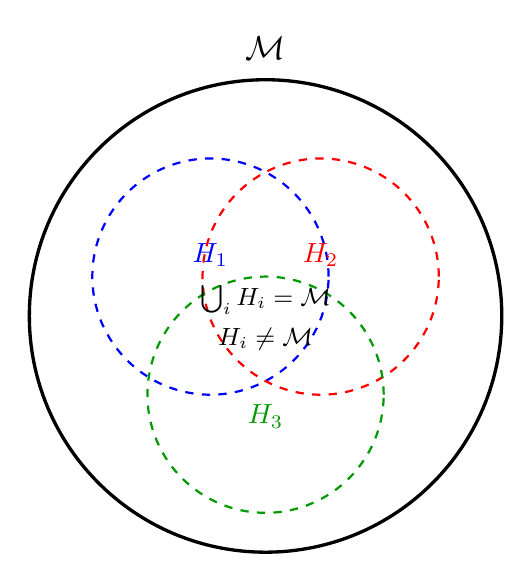
\begin{tikzpicture}
  % Monoturn
  \draw[very thick] (0,0) circle (3);
  \node at (0,3.4) {\large $\mathcal{M}$};
  % Observer horizons
  \draw[thick,blue,dashed] (-0.7,0.5) circle (1.5)
    node[above,blue] {$H_1$};
  \draw[thick,red,dashed] (0.7,0.5) circle (1.5)
    node[above,red] {$H_2$};
  \draw[thick,green!60!black,dashed] (0,-1.0) circle (1.5)
    node[below,green!60!black] {$H_3$};
  % Annotation
  \node at (0,0.2) {\small $\bigcup_i H_i = \mathcal{M}$};
  \node at (0,-0.3) {\small $H_i \neq \mathcal{M}$};
\end{tikzpicture}
\caption{The Monoturn $\mathcal{M}$ as a union of observer horizons.
         Each horizon $H_i \subsetneq \mathcal{M}$ is accessible to
         one observer.
         The Monoturn is the object whose complete reconstruction is
         obstructed by nontrivial admissibility cohomology
         $H^1(\mathcal{M},\mathcal{A}) \neq 0$
         (Conjecture~\ref{conj:cosmic-obstruction}).}
\label{fig:monoturn}
\end{figure}

\begin{CitationAnchor}
  The philosophical idea that every observer encounters reality
  through a limited perspective has a long history in
  phenomenology, from Husserl's concept of horizons to
  Merleau-Ponty's embodied perception.
  The mathematical formalisation here --- as sheaf cohomological
  obstruction --- is novel.
  Horizon limitations in cosmology are discussed in standard
  references such as Peebles~\cite{peebles1993} and
  Weinberg~\cite{weinberg2008}, though not in the sheaf-theoretic
  language developed here.
\end{CitationAnchor}

\begin{FurtherReading}
  For the philosophical background on horizons and limited
  observation, Ortega y Gasset's essay ``La perspectiva como
  forma de la realidad'' (1916) and Husserl's discussions of
  intentionality and horizon provide motivation.
  The mathematical theory of cosmic horizons is developed in
  Peebles~\cite{peebles1993}.
\end{FurtherReading}
